% !TEX root = ../../../../main/numb3rs_activities.tex
\newpage
\phantomsection
\addcontentsline{toc}{subsection}{102: Sabotage \label{ep102}}
\ep{102: Sabotage}


Don investigates a series of train wrecks that recreate accidents due to railroad negligence. A numerical code is left at the site of each accident. Charlie helps Don to find the terrorist behind the recreations by breaking the codes, which contain statistics of the wrecks occurred in the past.


The art of breaking codes by analyzing patterns is part of a wider mathematical area called Cryptography. In \hyperref[ep205]{Episode 205} the reader can find a brief explanation of some of the simplest algorithms to \emph{encode} and \emph{decode} information (we also refer the reader to \hyperref[ep324]{Episode 324}). In order to break the code in this episode, Charlie also uses \emph{statistical data analysis}, a technique mentioned in \hyperref[ep211]{Episode 211} as well.


By the end of the episode, Charlie gives a passionate speech about the way nature communicates to us in terms of mathematical patterns. We quote his exact words here: 
	\begin{center}
	\begin{minipage}{0.75\textwidth}
	\emph{``Math is the real world, okay, it's everywhere, okay. Can I show you? You see how the petals spiral? The number of petals in each row is the sum of the preceding two rows, the Fibonacci Sequence. It's found in the structure of crystals and the spiral of galaxies and a nautilus shell. What's more, the ratio between each number in the sequence to the one before it is approximately 1.61803, what the Greeks call the Golden Ratio. It shows up in the pyramids of Giza and the Parthenon at Athens, the dimensions of this card. And it's based on a number we can find in a flower. Math is nature's language\dots its method of communicating directly with us. Everything is numbers.''}
	\end{minipage}
	\end{center}


Below we will explain the main properties of the \textbf{Fibonacci sequence} and the \textbf{Golden Ratio}, and we will formally establish the relationship between these two mathematical entities.


% Fibonacci
\ltLarge{The Fibonacci Sequence}


\textcolor{CornellRed}{The Fibonacci sequence} is a sequence of numbers, $(F(n))_{n \geq 0}$, generated recursively in the following way,
	\[
	\begin{split}
	F(0)&= 0 \\
	F(1)&= 1 \\
	F(n)&= F(n-1) + F(n-2) \text{ for } n \geq 1.
	\end{split}
	\]


\tangent{\textbf{The Fibonacci sequence} or \textbf{Fibonacci numbers} are named after Leonardo of Pisa (about 1175--1250), who was nicknamed Fibonacci (from fillies Bonaccio, i.e. son of Bonaccio). He was investigating (in the year 1202) how fast rabbits breed in ideal circumstances and found out that the number of pairs of rabbits, female and male, in the population increases according to the mentioned sequence.}


In words, \textcolor{CornellRed}{every number in the sequence is equal to the sum of the two previous ones}. The numbers in this sequence get arbitrarily big as n increases. The first 11 numbers in this sequence are shown below:
	\[
	0, \quad 1, \quad 1, \quad 2, \quad 3, \quad 5, \quad 8, \quad 13, \quad 21, \quad 34, \quad 55\ldots\, .
	\]
Charlie mentions that this sequence is found in the spiral structure of some flowers and galaxies. Here we explain what he referred to. Suppose that you have two squares of side-length equal to \textcolor{CornellRed}{1}, sharing one of the sides. Then you put a square of side-length \textcolor{CornellRed}{2} on top of them. Then you draw a square of side-length \textcolor{CornellRed}{3} on the left of the rectangle drawn before. And you continue this way, adding squares of \textcolor{CornellRed}{side-length equal to the sum of the side-lengths of the two previous squares}, as shown in the figure on the right. Then, by construction, the lengths of the squares increase according to the Fibonacci sequence, and if you draw a curve joining the opposite vertices of the squares we obtain a spiral as shown in the figure as well.
	\begin{figure}[H]
	\centering
	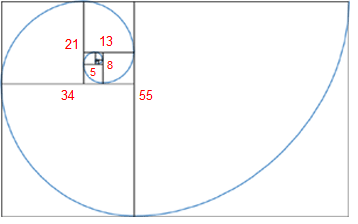
\includegraphics[width=0.5\textwidth]{../sections/seasons/season1/102/images/spiral.png} 
	\end{figure}
These spirals appear in nature in numerous examples, such as sea shells, flowers and galaxies. The reader can find more about the appearance of the Fibonacci sequence in nature at \lbref{http://www.maths.surrey.ac.uk/hosted-sites/R.Knott/Fibonacci/fibnat.html}


The Fibonacci numbers satisfy a numerous amount of very interesting identities. The reader can find some of them at \lbref{http://mathworld.wolfram.com/FibonacciNumber.html}. We will concentrate our attention here to its relationship with the golden ratio, which we explain below.


% Golden Ratio
\ltLarge{The Golden Ratio}


Suppose that you have a rectangle with sides of length 1 and x. Then you partition the rectangle into a square with side length 1 and another rectangle of side lengths 1 and x-1. The \textcolor{CornellRed}{golden ratio} or \textcolor{CornellRed}{golden proportion} is the only positive number x such that the two rectangles obtained by this construction are similar, i.e.
	\[
	\frac{x}{1}= \frac{1}{x-1}.
	\]

	\begin{figure}[H]
	\centering
	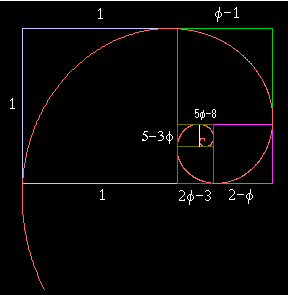
\includegraphics[width=0.5\textwidth]{../sections/seasons/season1/102/images/spiral2.png} 
	\end{figure}
The golden ratio is usually denoted by the Greek letter $\phi$, and according to the equation above we find that $\phi$ satisfies the following quadratic equation
	\[
	\phi^2 - \phi - 1 = 0,
	\]
which implies that $\phi= \dfrac{1 + \sqrt{5}}{2} \approx 1.61803398874989\cdots$. \\


This number possesses many nice properties. For instance its continued fraction representation (\hyperref[ep101]{Episode 101}) only contains ones, i.e.
	\[
	\phi= 1 +  \cfrac{1}{1 + \cfrac{1}{1 + \cfrac{1}{1 + \frac{1}{\;\;\ddots}}}}.
	\]


\tangent{The golden ratio or golden proportion was known by the ancient Greeks, it occurs in some of the Platonic Solids and it is mentioned in Euclid's Elements. Although this golden proportion is found in some of the Ancient Greek constructions, such as the Parthenon, there is no definite evidence that they were designed by using this mathematical constant (see picture below). The reader can find more about the golden ratio and architecture at Dr. Ron Knott's website.}


There is also a nice way of expressing the golden ratio as a limit of radicals in the following way,
	\[
	\phi= \sqrt{1+\sqrt{1+\sqrt{1+\sqrt{1+\cdots}}}}
	\]
Regarding the construction at the beginning of the section, if we continue partitioning the successive rectangles into a square and a new rectangle, we deduce that all the rectangles are similar, and if we draw a curve joining the opposite vertices of the squares we obtain a spiral similar to the one generated by the Fibonacci sequence. Below we explain the algebraic relationship between the golden ratio and the Fibonacci sequence, which explains the similarity of the mentioned spirals, \bref{The Golden Section in Architecture}{http://www.maths.surrey.ac.uk/hosted-sites/R.Knott/Fibonacci/fibInArt.html}. 


% Golden & Fib.
\ltLarge{The Relationship Between the Golden Ratio and the Fibonacci Sequence}


The quadratic formula satisfied by the golden ration implies that
	\[
	\phi^2=\phi+1 \longrightarrow \phi^n=\phi^{n-1}+\phi^{n-2} \text{ for } n \geq 2
	\]

	\begin{figure}[H]
	\centering
	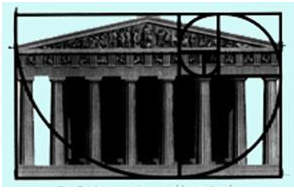
\includegraphics[width=0.5\textwidth]{../sections/seasons/season1/102/images/parthenon.png} 
	\end{figure}


Since $1-\phi= - \phi^{-1}$ satisfies the same equation, we get that
	\[
	(1-\phi)^n= (1 - \phi)^{n-1} + (1 - \phi)^{n-2} \text{ for } n \geq 2.
	\]
Define
	\[
	\widetilde{F}(n)= \frac{\phi^n - (1 - \phi)^n}{\sqrt{5}}= \frac{\phi^n - (-\phi)^{-n}}{\sqrt{5}}.
	\]
The two facts above imply that  $(\widetilde{F}(n))_{n \geq 0}$ satisfies the Fibonacci recursion as well and since
	\[
	\begin{split}
	\widetilde{F}(0)&= 0 \\
	\widetilde{F}(1)&= \frac{\phi - (1 - \phi)}{\sqrt{5}} = \frac{2\phi - 1}{\sqrt{5}} = 1.
	\end{split}
	\]
We conclude that $\widetilde{F}(n)=F(n)=\dfrac{\phi^n-(1-\phi)^n}{\sqrt{5}}=\dfrac{\phi^n-(-\phi)^{-n}}{\sqrt{5}}$. 


\tangent{Binet's formula is named after the French mathematician Jacques Philippe Marie Binet, who derived it in 1843. However, this formula was already known by Euler, Daniel Bernoulli, and de Moivre more than a century earlier.}


This is the famous \textcolor{CornellRed}{Binet's formula}, which gives us a closed expression for the terms of the Fibonacci sequence in terms of n. This formula allows us to prove properties of the Fibonacci sequence, in particular we can prove that,
	\[
	\lim_{n \to \infty} \frac{F(n+1)}{F(n)} = \lim_{n \to \infty} \frac{\phi^{n+1} - (1-\phi)^{n+1}}{\phi^n - (1 - \phi)^n} = \phi.
	\]
This formula in words tells us that as $n$ increases, the ratio between consecutive terms of the Fibonacci sequence approaches the golden ratio. This is exactly what Charlie is referring to when he says: ``\dots the ratio between each number in the sequence to the one before it is approximately $1.61803$, what the Greeks call the Golden Ratio.''